
\section{Aufbau}
\label{sec:Aufbau}

Der Versuch wird wie in Abbildung \ref{fig:Aufbau} aufgebaut. Am Rezipient (B1) wird über ein Kreuzstück (B2) ein Nadelventil (D1) für die Leckratenmessung der Drehschieberpumpe und alle Messungen der Turbomolekularpumpe angebracht. Über ein Kugelventil (V3) kann dieses komplett geschlossen werden. Über ein T-Stück wird ein Kaltkathoden-Vakuummeter angeschlossen, welches in der Abbildung links nicht zu sehen ist. Über ein weiteres T-Stück (B3) mit eingebautem Heizkathoden-Vakuummeter (H1) und ein Klappenventil (V1) wird der Rezipient mit der Turbopumpe verbunden. Mit einem Kugelventil (V2) wird der Tank außerdem über die Schläuche (S1) und (S2) mit der Drehschieberpumpe verbunden, die ebenfalls zur Erzeugung des Vorvakuums der Turbopumpe verwendet wird. Dazu ist die Drehschieberpumpe über ein kleines Kreuzstück (B5) und ein Kugelventil (V5) mit der Turbopumpe verbunden. Über ein T-Stück (B6) sind ein analoges und ein digitales Pirani-Vakuummeter (P1 und P2) angeschlossen. Letzteres war bei dieser Durchführung des Versuchs defekt.

\begin{figure}
\begin{minipage}{0.5\textwidth}
	\centering
	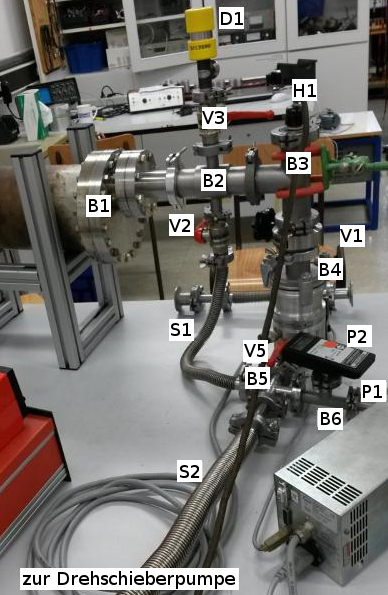
\includegraphics[width=0.9\textwidth,keepaspectratio]{content/images/Aufbau2.jpg}
\end{minipage}
\begin{minipage}{0.5\textwidth}
	\centering
	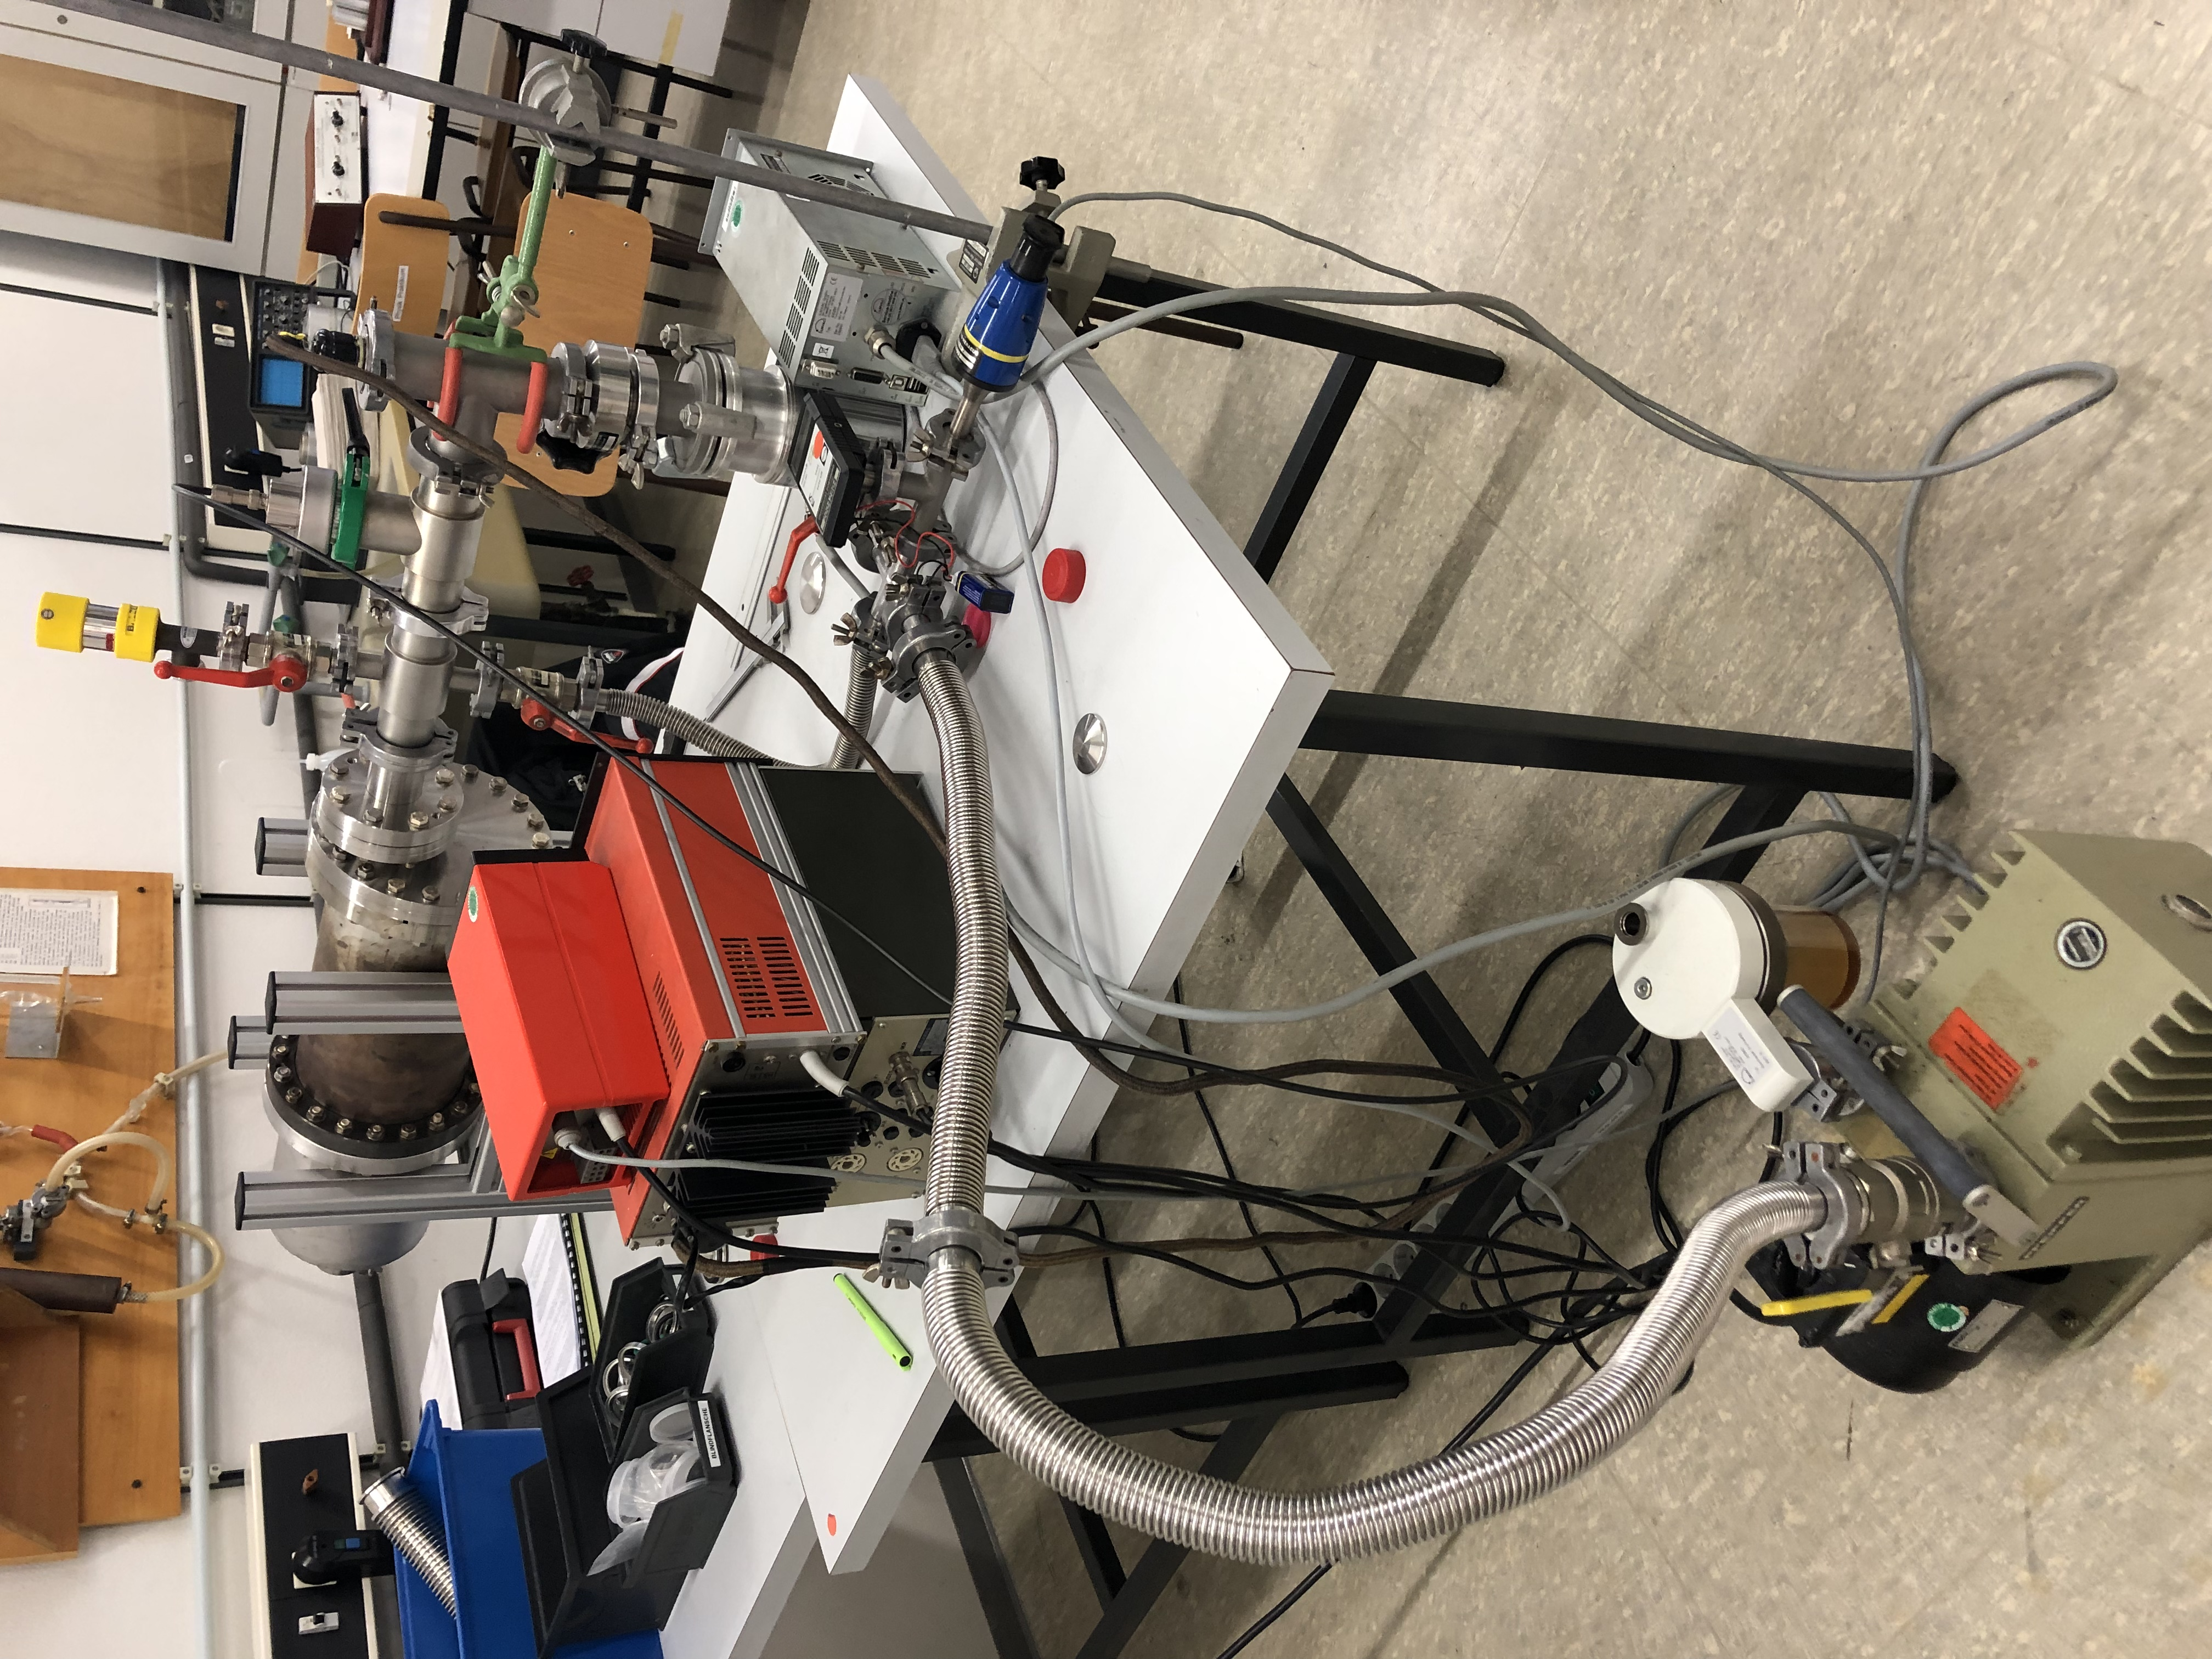
\includegraphics[width=0.9\textwidth,keepaspectratio]{content/images/Aufbau3.jpg}
\end{minipage}
\caption{Versuchsaufbau.}
\label{fig:Aufbau}
\end{figure}

